\section{Results}
In this Section, we first discuss the results of Python Idioms we tested on \cop{}. We then discuss the results of Best Practices in Javascript using the methodology described in Section~\ref{methodology}.

\subsection{Pythonic Idioms}
\label{secidioms}
The definition for the term \emph{Pythonic} in Python can be found in official Python glossary\footnote{\url{https://docs.python.org/3/glossary.html\#term-pythonic}}:

\begin{quote}
    An idea or piece of code which closely follows the most common idioms of the Python language, rather than implement- ing code using concepts common to other languages. For example, a common idiom in Python is to loop over all elements of an iterable using a for statement. Many other languages do not have this type of construct, so people unfamiliar with Python sometimes use a numerical counter instead, as opposed to the cleaner, pythonic method.
\end{quote}

This definition indicates a broad meaning, referring to both concrete code, but also \emph{Ideas} in general sense. Many Python developers argue that coding the \emph{pythonic way} is the most accepted way to code by the Python community~\cite{Alexandru2018}. We consider an \emph{idiom} to be any reusable abstraction that makes Python code more readable by shortening or added syntactic sugar. Idioms can also be more efficient than a basic solution and some idioms are both more readable and more efficient.

We sampled idioms from the work of Alexandru et al.~\cite{Alexandru2018}, which identified idioms from presentations given by renowned Python developers that frequently mention Idioms, e.g., Hettinger~\cite{hettinger} and Jeff Knupp~\cite{knupp} and popular Python books, such as ``Pro Python''~\cite{Alchin2010}, ``Fluent Python''~\cite{fluent}, ``Expert Python Programming'' by Jaworski and Zaide~\cite{expert}.

Using the methodology described in Section~\ref{methodology}, we picked the top 10 most popular Python Idioms from work of Alexandru et al.~\cite{Alexandru2018} and checked if \cop{} suggests the optimal way. \cop{} suggested the ideal approach as the first suggestion in 2 of the 10 idioms we tested i.e, Copilot did not have the recommended way as its top suggestion. However, 4 out of those remaining 8 Idioms had the Ideal way in \cop{} top 10 suggestions currently viewable. 

Table~\ref{tab:all_idioms} shows complete the list of all the Idioms we tested and the ranking of the Ideal way in \cop{} suggestions (if it exists).

\renewcommand{\arraystretch}{1.5}
\begin{table}[ht]
    \centering
    \begin{tabular}{|L|c|}
    \hline
         \textbf{Idiom Title} & \textbf{\cop{} Suggestion Matched?} \\
         & (out of 10 suggestions) \\
         \hline
         List Comprehension & No \\
         \hline
         Dictionary Comprehension & No \\
         \hline
         Mapping & 9\textsuperscript{th} \\
         \hline
         Filter &  7\textsuperscript{th} \\
         \hline
         Reduce & 9\textsuperscript{th} \\
         \hline
         List Enumeration & No \\
         \hline
         Set Comprehension & 1\textsuperscript{th} \\
         \hline
         Read and Print from a file & 5\textsuperscript{th} \\
         \hline
         Add int to all list numbers & No \\
         \hline
         If condition check value & 1\textsuperscript{th} \\
         \hline
    \end{tabular}
    \caption{List of all Python Idioms tested on \cop{}.}
    \label{tab:all_idioms}
\end{table}

Figure~\ref{fig:idioms_1} shows the List Comprehension idiom, showing user input (i.e., Human Input), the top suggestion by \cop{} and the recommended way suggested by Alexandru et al.~\cite{Alexandru2018}.


All the Idioms shown in Table~\ref{tab:all_idioms} can be found in the \repl{} including the code used as input (i.e., Human Input), the top suggestion by \cop{} and the Ideal Way.

% \begin{tcolorbox}[title=List Comprehension,boxsep=.25mm]
%     %https://tex.stackexchange.com/questions/337909/tcolorbox-tcbline-style
% \textbf{Human Input:}
% \begin{lstlisting}[language={Python}]
% #list comprehension
% result_list = 
% \end{lstlisting}
% \tcbline
% \textbf{Copilot Suggestion:}
% \begin{lstlisting}[language=Python,escapechar=\%]
% % \noindent\textcolor{gray}{result\_list  =} % []
% for i in range(1,11):
%     result_list.append(i)
% \end{lstlisting}
% \tcbline
% \textbf{Ideal way\footnote{source \cite{Alexandru2018}}:}
% \begin{lstlisting}[language=Python]
% result_list = [el for el in range(11)]
% \end{lstlisting}
% \end{tcolorbox}

%%%%%% TODO: remember to update the screenshot if the source citation is different from the citation in the text %%%%%%
\begin{figure}[hbt!]
    \centering
    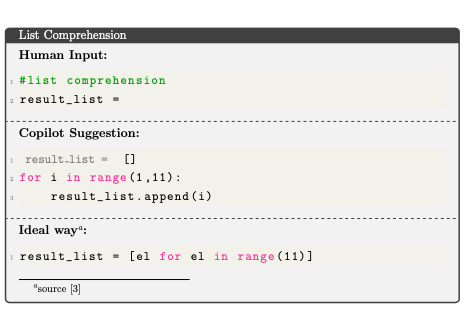
\includegraphics[width=\linewidth]{Figures/idioms_1.png}
    \caption{List Comprehension Idiom and \cop{} Suggestion}
    \label{fig:idioms_1}
\end{figure}
